\documentclass{article}
\usepackage{graphicx}
\usepackage{microtype}
\usepackage[numbers]{natbib}

\graphicspath{
	{pictures/}
}

\renewcommand{\contentsname}{Tartalomjegyzék}
\renewcommand{\figurename}{Ábra}
\renewcommand{\listfigurename}{Ábrajegyzék}
\renewcommand{\tablename}{Táblázat}
\renewcommand{\listtablename}{Táblázatok jegyzéke}

\begin{document}
	\title{Nyári gyakorlatos beszámoló - államvizsga}
	\author{Nagy-Serbán Tünde Számítástechnika III. év}
	\maketitle
	
	\newpage
	
	\tableofcontents
	
	\listoffigures
	
	\listoftables
	
	\newpage
	
	\section{Bevezető}
	\label{sec:bevezeto}
	\paragraph{}
	A mai gyorsan fejlődő világunkban a digitális eszközök kezdik átvenni az uralmat. Nem sok olyan háztartás van ahol nincs egyáltalán legalább egy telefon, számítógép, laptop, okos tv stb. Az elmúlt években a digitális világ annyira fejlett lett, hogy lassan már ki sem kell mozdulnunk a házból és mindent eltudunk végezni. Például ki tudjuk fizetni a számláinkat, be tudunk vásárolni stb. Ezek mellett egyes múzeumokat, iskolákat, kastélyokat, látványosságokat is betudunk járni otthon a négy fal között a 3D túrák segítségével. De mit is jelent, mire is használják ezeket a 3D túra modelleket?
	\paragraph{}
	A 3D jelentése három dimenzió. Ez egy modell, amely tulajdonképpen matematikailag ábrázol egy háromdimenziós objektumot. Ez lehet épület, virág, ember stb. A 3D modelleket széles körben használnak az orvostudományban, magasabb szintű gyakorlati és elméleti kompetenciák elérésére. A 3D modellekkel nem csak tárgyakat hanem emberi folyamatokat is le lehet szimulálni. Az orvos tudományban nagyon szépen letudják előre játszani az operációkat így biztosabban fognak neki az adott műtétnek mivel jobban tudják kezelni a kockázatokat. Ilyen modellek felhasználásával egy adott problémát is jobban betudnak mutatni az emberek számára. Ilyen példa lehet egy hajóforgalom szimulációs rendszer amely figyelembe veszi a hajókat, vízfelületet és az időjárási viszonyokat. Ezzel a rendszerrel \cite{dedov2017design} próbálták megmutatni az olajszennyezést a tengerekben, óceánokban. Ezen modellek segítségével a világ látványosságai elérhetővé válhatnak azon emberek számára is akik nem jutnak el az eredeti országba, városba, hogy megtudják tekinteni az adott látványosságot.
	\paragraph{}
	A túra (tour) szó jelentése utazás, kirándulás. A mai világban túrázni nem csak a való életben lehet hanem a virtuális világban is. Egy ilyen virtuális túra célja, hogy fejlettebb szimulációs technikák segítségével a nézők életképes 3D-s képet kapjanak a meglévő helyről. Egy híres és megemlítendő példa a Second-Life ahol a felhasználók közötti interakció avatárokon keresztül zajlik. Ez azért megemlítendő példa mivel ezen alkalmazáson belül interaktív 3D túrák vannak leképezve.\cite{moloo20163d}
	\paragraph{}
	A 3D és a túra(tour) szavak összetételéből jön ki a 3D túra(3D tour) amely azt tükrözi, hogy a virtuális világban tudunk megnézni adott épületeket, kilátásokat, látványosságokat. Világunk fejlődése próbálja biztosítani, hogy egyetlen ember se maradjon le azon helyekről ahová nem tud eljutni. Habár ezen virtuális 3D modelleken alapuló világ még nem tökéletes de folyamatosan fejlődik. A dolgozatomon belül egy ilyen modellről lesz szó amely a Sapientia Erdélyi Magyar Tudományegyetem Marosvásárhely-i karának egy részét tartalmazza. A projekt két részre van bontva. Egy személy készíti el maga a modellt míg egy másik társ a felhasználói felületet. Ezen dolgozatban a felhasználói felületről lesz inkább szó. 
	\paragraph{}
	A projekt célja, hogy a felhasználók a saját házukból is betekintést tudjanak nyerni az egyetem falai mögé is. Ez elsősorban az új felvételizőknek és az első éves egyetemistáknak lenne hasznos, mivel ez által már otthon neki foghatnak áttekinteni az egyetem különböző részeit mint például, hogy hol található egy adott tanszék, vagy hol található a dékáni hivatal, vagy hogy hol található a pénztár. Úgy gondolom, hogy ez az alkalmazás hasznos tud lenni a diákok részére sőt a szakkoordinátorok dolgát is megtudja annyiban könnyíteni, hogy az újonnan érkező diákok nem kell mindig hozzájuk forduljanak, hogy hol találnak meg egy adott részleget.
	\paragraph{}
	Több okot is fellehet sorolni annak érdekében, hogy miért is használatosak ezek a 3D modellekkel megalkotott túrák. Első sorban az új diákok már otthonról be tudnak nézni az egyetem falai mögé így amikor elérkeznek az új év kezdéséhez akkor otthonosabban érezhetik magukat. Ez azért történhet meg mert már fogják tudni, hogy mit hol találnak nem kell segítséget kérjenek. Egy másik ok, hogyha az adott egyetem rendelkezik egy ilyen típusú modellel akkor jobban felhívhatja a figyelmet a diákok számára. Ez által az egyetem népszerűsítése is megtörténik. Ismert, hogy egyes szülők nehezen engedik el gyermeküket egyetemre mert féltik. Viszont az, hogy látnak egy  képet az egyetemről megnyugtathatja őket így bátrabban biztathatják gyermeküket, hogy menjen el az adott egyetemre. 
	\paragraph{}
	Összefoglalva egy ilyen 3D modell amely az egyetemet ábrázolja és bemutatja hasznos lehet, az egyetem, a diákok és szüleik számára is. Egy ilyen alkalmazás esetében nem csak maga a modell jelenik meg hanem rajta kívül számos fontos információ, elérhetőség is. Dolgozatom célja bemutatni a Sapientia Erdélyi Magyar Tudományegyetem 3D Virtual Tour alkalmazás megalkotását, implementálását és nem utolsó sorban a felhasznált technológiákat.
	
	\newpage
	
	\section{Technológiai áttekintés}
	
	\subsection{Adatbázisok}
	\paragraph{}
	Adatbázisnak nevezzük azokat a nagy mennyiségű adatokat amelyek közös jellemzőkkel és struktúrákkal rendelkeznek. Az adatbázisokon belül több fajta műveletet tudunk elvégezni: karbantartás, tárolás, lekérdezés, szerkesztés, módosítás és nem utolsó sorban az adatok törlése is egy lehetőség. Ezen funkciókat egy adatbázis kezelő rendszer segítségével tudjuk elvégezni.\cite{dbms} Azonban különbséget kell tennünk az SQL (Structured Query Language) és a NoSQL(Not only Structured Query Language) között.
	\subsubsection{SQL(Structured Query Language)}
	\paragraph{}
	Az elmúlt harminc évben a relációs adatbázis volt az alapértelmezett strukturált adatlekérdezési nyelv. Világunk fejlődése miatt egyre több és nagyobb információ adatok robbantak ki így az SQL alapú adatlekérdezés elveszítette hatékonyságát ezzel maga elé állítva azt a kihívást, hogy a nagyobb adatbázisok kezelése jóval megnehezedett. Ebből kifolyólag lehet arra következtetni hogy az SQL alapú szerverek hajlamosak nagy mennyiségű memóriát foglalni, biztonsági kockázatokat és teljesítményproblémákat elkövetni.\cite{venkatraman2016sql} 
	
	\subsubsection{NoSQL(Not only Structured Query Language)}
	\paragraph{}
	A NoSQL adatbázisokat azért alkották meg, hogy az SQL adatbázisok által felfedezett hibákat orvosolják. Ezek az adatbázisok sokkal rugalmasabbak lettek, fő céljuk az adatok könnyű tárolása és visszakeresése függetlenül a szerkezetektől és tartalomtól. Automatikusan kezelik az adatkezelést, hibajavítást amelyek költségmegtakarítás szempontjából is fontosak.\cite{venkatraman2016sql} 
	
	\subsubsection{SQL vs NoSQL}
	\paragraph{}
	A relációs adatbázisok az egyszerűség miatt leggyakoribb adatbázistípusok. Az adatok több táblára vannak bontva amelyekhez egyszerűen hozzá lehet férni. Az olyan műveletek, mint összeadás, létrehozás, visszakeresés, törlés stb. nagyon egyszerűen elvégezhetőek az SQL által megadott szintaxisok betartásával. Ilyen típusú adatbázis kezelő rendszerek a következőek: Oracle, SQL Server, MySQL, PostgreSQL stb. A folyamatos adatmennyiség miatt a relációs adatbázisok hátrányba kerültek a nem relációs adatbázisokkal szemben. A nem relációs adatbázisok sokka gyorsabban és hatékonyabban tudják elvégezni feladatikat mint a relációsak. Nem reláció adatbázis típsú rendszerek a következőek lehetnek: Firebase, MongoDB, GraphQL stb.\cite{gupta2017nosql} A tanulmányok sokat segítenek abban, hogy egy adott projektben relációs vagy nem relációs adatbázist használjunk. Ha sok adatunk van és törekedünk a hatékonyságra akkor érdemesebb a nem relációs adatbázisokat használni. 
	\paragraph{}
	Több tanulmány is szól az adatbázisok teljesítményéről. A következőkben bemutatnék egyet. Ebben a tanulmányban három tesztet végeztek el. A kísérletben szerepelnek a következő adatbázis kezelő rendszerek: Cassandra, HBase, Memcached, MongoDb, OrientDB, Redis és a Voldemort.\cite{martins2019study} Az első tesztben 6.000.000 rekord állt az adatbázis kezelők rendelkezésére. A munkaterhelés fele olvasást és fele frissítést tartalmazott. Az eredmény a \ref{fig:performance_a} ábrán látható.
	
	\begin{figure}
		\centering
		\frame{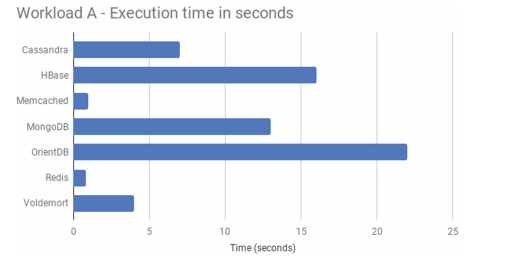
\includegraphics[width=0.8\linewidth]{performance_a}}
		\caption{Az adatbázis teljesítmény kísérlet első eredménye \cite{martins2019study}}
		\label{fig:performance_a}
	\end{figure}

	A második teszt szintén 6.000.000 rekordot tartalmazott. A munkaterhelés 5.000 véletlenszerű olvasás volt. Az eredmények \ref{fig:performance_b} ábrán láthatóak.
	
	\begin{figure}
		\centering
		\frame{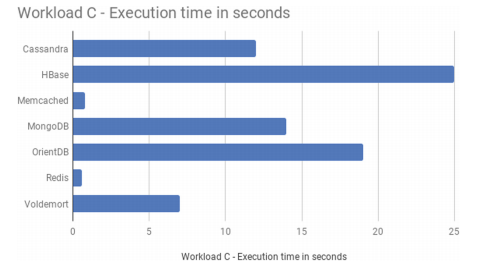
\includegraphics[width=0.8\linewidth]{performance_b}}
		\caption{Az adatbázis teljesítmény kísérlet második eredménye \cite{martins2019study}}
		\label{fig:performance_b}
	\end{figure}
	
	A harmadik teszt szintén 6.000.000 rekordot tartalmazott. A munkaterhelés 5.000 véletlenszerű frissítés volt. Az eredmények \ref{fig:performance_c} ábrán láthatóak.
	
	\begin{figure}
		\centering
		\frame{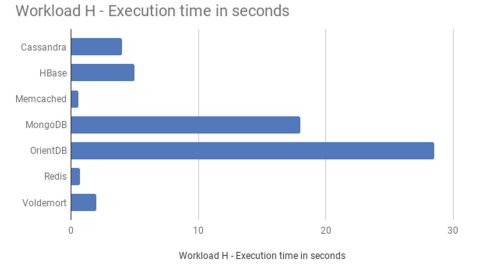
\includegraphics[width=0.8\linewidth]{performance_c}}
		\caption{Az adatbázis teljesítmény kísérlet harmadik eredménye \cite{martins2019study}}
		\label{fig:performance_c}
	\end{figure}
	
	\subsection{Keretrendszerek}
	\paragraph{}
	A keretrendszereket szoftvermérnökök és programozók készítik, tesztelik és optimalizálják. Ezek a rendszerek sokoldalúak, robusztusak és hatékonyak. A különböző alkalmazások fejlesztéséhez az ilyen jellegű rendszerek segítségével csak a magasabb szintű funkcionalitások elvégzésére kell koncentrálni. Erre az a magyarázat, hogy a keretrendszer gondoskodik az alacsonyabb funkcionalitásokkal. Számos előnyt lehet felsorolni, hogy miért jó ha használjuk ezeket a rendszereket.\cite{frameworks}
	\begin{itemize}
		\item Elősegíti a tervezési minták megfelelő kialakítását.
		\item Biztonságosabb kódolás.
		\item A redundáns kód elkerülése.
		\item Következetes kódfejlesztés kevesebb hibával.
		\item Megkönnyíti a kód tesztelését és a hibakeresést is.
		\item Az alkalmazás fejlesztéséhez szükséges idő lecsökken.
	\end{itemize}

	\subsubsection{Angular}
	\paragraph{}
	Az Angulart 2008-ban kezdték el fejleszteni a Google munkatársai. A fejlesztés JavaScriptben történt. Abban az időben a webhelyek többsége többoldalas alkalmazás megközelítésén alapult. Ennek viszont a teljesítménye az idő elteltével romlani kezdett mivel befolyásoló tényező lett az internet kapcsolat és a szerver reakció képessége is. Ezért létre hozódott az egy oldalas alkalmazások megközelítése ami abban segít, hogy a több oldalas weboldalak csupán egy oldalon jelennek meg. Az Angular volt az egy oldalas alkalmazások első kerete. Az egyik fő előnye a megközelíthető jellege. Az sem elhanyagolható, hogy a fejlesztők egy részletes és egyértelmű dokumentációval szolgáltak a felhasználóknak. Egy TypeScript nyelv amely hasznos és könnyen használható. Megvan a saját szintaktikája viszont a fordítás során egyszerű JavaScript kódba fog átmenni.\cite{wohlgethan2018supportingweb}
	
	\subsubsection{Vue.js}
	\paragraph{}
	A Vue.js(röviden: Vue) tekinthető a legújabb keretrendszernek. Hasonlít az Angularhoz. Mindkéttő TypeScript típusú. Használható kisebb, egyszerűbb projekteknél és egy komplexebb egy oldalas alkalmazás elkészítésénél is. Fő érdeme a skálázhatóság. Különlegessége, hogy egy nyílt forráskódú közösség fejlesztette ki, nem pedig egy nagyobb válalat. Egy komponens alapú keretrendszer. Azt jelenti, hogy komponenseket különböztetünk és jelenítünk meg. Egy komponensen belül tudunk írni HTML, CSS és Script elemeket is. A megjelenítés egy oldalon történik ezért szükséges használni a útválasztást(rout).\cite{wohlgethan2018supportingweb}
	
	\subsubsection{Angular vs Vue.js}
	\paragraph{}
	Mindkét keretrendszernek megvannak az előnyei \ref{tab:table1} táblázat és a hátrányai is \ref{tab:table2} táblázat. 
	\begin{table}
		\begin{center}
			\caption{Előnyök Angular és Vue.js között \cite{vuevsang} }
			\label{tab:table1}
			\begin{tabular}{c|c|c} 
				\textbf{Sorszám} & \textbf{Angular} & \textbf{Vue.js}\\
				\hline
				1 & TypeScript használata & TypeScript használata, részletes dokumentáció\\
				\hline
				2 & Részletes dokumentációval rendelkezik & Egy oldalas alkalmazások készítése \\
				\hline
				3 & Gyorsítja a fejlesztést & Könnyű integráció a meglévő struktúrákba \\
				\hline
				4 & & Kihasználja virtuális DOM előnyeit \\
				\hline
				5 & & Sebessége és rugalmassága optimális \\
			\end{tabular}
		\end{center}
	\end{table}

	\begin{table}
		\begin{center}
			\caption{Hátrányok Angular és Vue.js között \cite{vuevsang}}
			\label{tab:table2}
			\begin{tabular}{c|c|c} 
				\textbf{Sorszám} & \textbf{Angular} & \textbf{Vue.js}\\
				\hline
				1 & Számos különféle struktúrát kínál, nehezíti a tanulást & Kevesebb erőforrást kínál\\
				\hline
				2 & Lassabb teljesítmény mert működik a reális DOM &  \\
			\end{tabular}
		\end{center}
	\end{table}
	\paragraph{}
	Az előnyöket és hátrányokat figyelembe véve kerestem egy ábrát amely megmutatja, hogy a Vue.js és az Angular mennyire használatosak. \ref{fig:vueang} ábra figyelembe veszi az érdeklődés és elégedettségi arányokat. A bemutatott adatok alapján mindkét keretrendszert sokan használják. Javasolt a Vue.js egy komplexebb, összetettebb projekt megvalósítása esetén viszont Angularral is ellehet készíteni. Mindkettővel frontend részt készítenek a fejlesztők.
	
	\begin{figure}
		\centering
		\frame{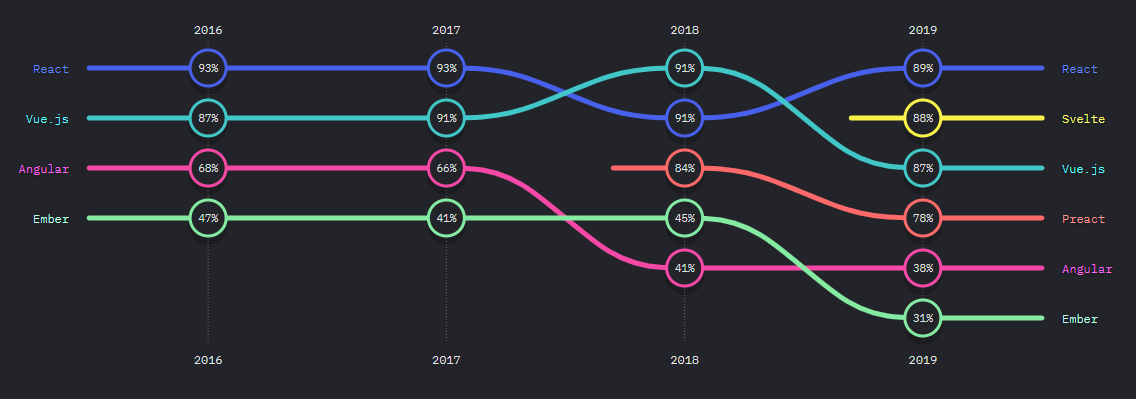
\includegraphics[width=0.8\linewidth]{vueang}}
		\caption{Keretrendszerek használatossága évekre bontva \cite{vueanginterest}}
		\label{fig:vueang}
	\end{figure}
	
	\subsubsection{NodeJs}
	\paragraph{} 
	A NodeJs egy olyan szoftver platform, amely a Chrome V8 JavaScript futási idején épül fel. Fontos tulajdonsága, hogy skálázható ezért is sokan használják. Eseményvezérelt, nem blokkoló I/O modellt használ, amely könnyűvé és hatékonnyá teszi a valós idejű alkalmazásokhoz, amelyek elosztott rendszeren futnak át. Használatos mivel aszinkron és a tanulási görbéje is helyeén van. A fejlesztők hatalmas köre már évek óta ismeri a JavaScriptet és az aszinkron programozást. Inkább támogatja a NoSQL adatbázisokat.\cite{js2016node}
	
	
	\subsubsection{Spring Boot}
	\paragraph{}
	A Spring Boot célja a Spring alkalmazás fejlesztés egyszerűsítése. Megtalálhatóak benne a következő tulajdonságok:
	\begin{itemize}
		\item Automatikus konfigurációk - az alkalmazások Springként való működése érdekében.
		\item Indítófüggőségek - szükséges függőségek automatikus integrálása.
		\item Parancssori tolmács.
		\item Működtetés - a consolba megjelennek az alkalmazás működésével kapcsolatos információk.
	\end{itemize}
	
	\paragraph{}
	Radikálisan gyorsabb és széles körben hozzáférhető, érhető Spring fejlesztést nyújt. Számos funkciót kínál: beágyazott szervereket, metrikákat, ellenőrzéseket, külső konfigurációkat. Saját struktúrával rendelkezik és mivel JSON fájlokon keresztül kommunikál nem tesz különbséget az adatbázisok között. A JAVA nyelvet használja.\cite{jovanovic2017java}
	
	\subsubsection{NodeJs vs Spring Boot}
	\paragraph{}
	NodeJs a következő különlegességeket tartalmazza \cite{nodejsspring}:
	\begin{itemize}
		\item A NodeJS alkalmazások fejlesztésének elindítása könnyű.
		\item Az agilis fejlesztési módszertant követi, amely alkalmas a nagyon skálázható alkalmazásfejlesztési szolgáltatásokra.
		\item Nagy projekteknél gyorsabban működik mint a Java.
		\item Hatalmas erőforrás-készlet könyvtárakkal rendelkezik
	\end{itemize}
	
	\paragraph{}
	Spring Boot a következő különlegességeket tartalmazza \cite{nodejsspring}:
	\begin{itemize}
		\item Egyszerű és minden eszköz és operációs rendszer támogatja.
		\item Beépített nyelvbiztonsági funkciókkal rendelkezik, amelyeket a Java Compiler beágyaz.
		\item Robusztus kódot alkalmaz.
		\item Integrációs képesség jó.
		\item Az alkalmazások egyszerűen építhetőek fel.
		\item Beágyazott HTTP-kiszolgálókat, például Jetty, Tomcat használ és egyszerűen teszteli a webes alkalmazásokkal.
	\end{itemize}
	
	\paragraph{}
	A fent leírtakat figyelembe véve kerestem egy ábrát \ref{nodespring} amely az érdekeltségi szinetet mutatja meg. \cite{nodejsspring1} Mindkét keretrendszert inkább backend fejlesztésére használják.
	
	\begin{figure}
		\centering
		\frame{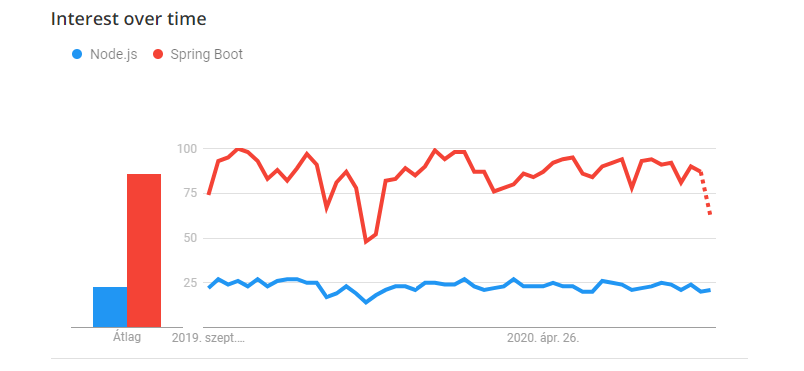
\includegraphics[width=0.8\linewidth]{nodespring}}
		\caption{NodeJS és SpringBoot érdekeltségi szintje}
		\label{nodespring}
	\end{figure}
	
	\newpage
	\section{Nyári fejlesztés}
	
	\subsection{Célkitűzések}
	\paragraph{}
	Az alkalmazás elkészítése érdekében szükséges volt elgondolkodni, hogy mit is szeretnék ezzel az alkalmazással nyújtani a nagy világnak. Melyek azok a fontos elemek, amelyekre mindenképpen szükség van egy ilyen jellegű alkalmazáson belül.
	\paragraph{}
	Elsődleges célom az volt, hogy az alkalmazás ne legyen bonyolult. Legyen minél egyszerűbb, átláthatóbb, használhatóbb. Hiszem azt, hogy egy egyszerűbb rendszer használatosabb mint egy bonyolultabb.
	\paragraph{}
	Elgondolkodtam azon is, hogy szükséges-e regisztráció majd bejelentkezés minden felhasználó részére. Idővel rájöttem, hogy ez nem szükséges hiszen ez az alkalmazás mindenki számára is nyitott kell legyen, mivel az a cél, hogy megmutassuk az egyetemet belülről. Így a regisztrációs ötlet részt teljesen elvetettem.
	\paragraph{}
	Habár a regisztrációs részt teljesen elvetettem eszembe jutott, hogy az alkalmazáson néha kell frissíteni ezért kellenek egyedi felhasználók is amelyek elérik az alkalmazás azon részeit amit a közönséges felhasználó nem. Így jött az ötlet, hogy csak kimondottan bejelentkezés lesz és az új nem általános felhasználókat egy adott státusszal rendelkező admin felhasználó tud hozzá rendelni.
	\paragraph{}
	Az egyedi felhasználók szempontjában is a legnagyobb cél az átláthatóság, egyszerűség, könnyen kezelhetőség. Ennek érdekében az a cél, hogy minden egyedi felhasználó számára csak az elérhető módosítási lehetőségek jelenjenek meg. 
	\paragraph{}
	A bejelentkező személyek számára biztosítani szeretném, a felhasználói adatok biztonságos eltárolását és kezelését is.
	\paragraph{}
	Célom az is, hogy az egyetemről minél több információ kerüljön be az alkalmazásba. Ezt úgy kell érteni, hogy az adott tanszékekről, szakokról egy bővebb leírást mutatni, ezáltal a diákok jobban eltudják dönteni, hogy az a szak amelyet kiválasztanak mennyire lesz jó számukra.
	\paragraph{}
	Mivel az alkalmazás első éves diákok számára készül és ők még nem ismerik az egyetem keretein belül szervezendő eseményeket sem, így az is a célok közé tartozik, hogy egy esemény naptárral is bővüljön az alkalmazás. Így az új diákok tisztában lehetnek, hogy milyen események lesznek, fogják tudni a helyszínt és dátumot is.
	\paragraph{}
	Szeretnék, egy olyan részt is biztosítani minden felhasználó számára ahol a saját véleményét tudja kifejteni. Ezen véleményeket figyelembe véve szeretném kijavítani az észlelt hibákat.
	
	\subsection{Funkcionalitások}
	\paragraph{}
	Alkalmazásomon belül több fajta funkcionalitás jelenik meg. Első sorban nincs regisztrációhoz kötve a felhasználó. Ez azt akarja jelenteni, hogy mindenki előtt nyitva áll az alkalmazás, amelynek röviden leírt funkcionalitásai a \ref{fig:UseCaseEvery} ábrán lehet megtekinteni. Viszont vannak különleges joggal rendelkező felhasználók, akik be tudnak jelentkezni és ennek következtében több funkcionalitást képesek használni. Ezen funkciónalítások a \ref{fig:UseCaseAdmin} ábrán láthatóak.
	
	\begin{figure}
		\centering
		\frame{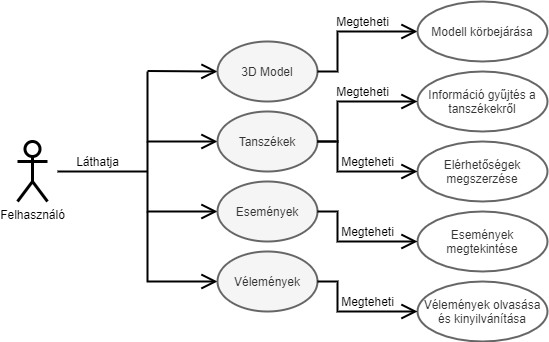
\includegraphics[width=0.5\linewidth]{UseCaseEvery}}
		\caption{Use Case diagram általános felhasználók számára}
		\label{fig:UseCaseEvery}
	\end{figure}

	\begin{figure}
		\centering
		\frame{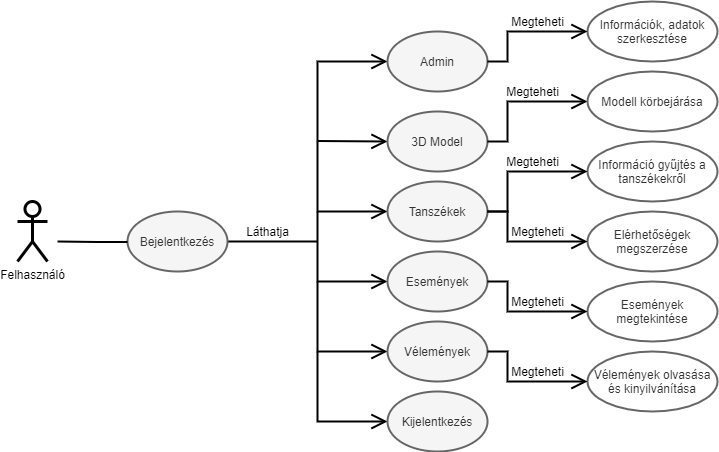
\includegraphics[width=0.5\linewidth]{UseCaseAdmin}}
		\caption{Use Case diagram bejelentkező felhasználók számára}
		\label{fig:UseCaseAdmin}
	\end{figure}

	\paragraph{}
	Nézzük meg, hogy milyen más funkciókkal tudnak dolgozni azon emberek akiknek joga van bejelentkezni. Elsős sorban tisztázom, hogy a bejelentkező személyeket három csoportba különböztetem meg. Vannak admin, tanár és diák felhasználók. Az admin felhasználó elér minden funkcionalitást. Az a jellegzetessége, hogy új felhasználót csak ő tud hozzá adni és csak ő tud törölni is. A hozzáadás úgy történik, hogy megad minden adatot és egy gombra kattintva az új adatok bekerülnek az adatbázis rendszerben. Közben az új felhasználó fog kapni egy email-t amellyel eltudja fogadni a jelentkeztetést. Ügyelni kell, hogy az email érvényessége időhöz kötött. A törlés csak egyszerűen kiválasztással történik. Egyetlen felhasználó sem tudja törölni saját magát még az admin joggal rendelkezők sem.
	\paragraph{}
	A következőkben a tanár joggal rendelkező felhasználók lehetőségeit részletezem. Ezeknek az embereknek lehetőségük van hozzáadni új 3D modelleket az egyetemről, eseményeket, órarend linkeket és nem utolsó sorban az oldalon található fejléc képének módosítására is képesek. A tanszékek, szakok leírásának megadásai is lehetővé válik számukra. Sőt ha netán új szak indul azt is hozzá lehet adni.
	\paragraph{}
	A diák joggal rendelkezőknek van egyelőre a legkevesebb funkcionalitásuk. Ők csak eseményeket tudnak létrehozni. Feltevődhet az a kérdés, hogy akkor miért van szükség rájuk? A válasz erre a kérdésre, hogy egyszer is diákokkal kapcsolatos eseményeket egy diák jobban megtudja fogalmazni mint egy tanár. Másrészt az alkalmazás fejlesztés alatt van ezáltal valószínűleg lesznek még számukra funkcionalitások. 
	\paragraph{}
	A bejelentkező felhasználók számára természetesen van kijelentkező opció is. Ezen funkciók mellett a fejlesztés során, valószínűleg sokkal több lesz. Egyelőre a cél az egyszerűségben rejlik. Tudni kell, hogy a modellnél, tanszékeknél, szakoknál és más fontos információknál elérhetőségeknél mindig az adatbázisban szereplő legújabb adat jelenik meg. 
	\paragraph{}
	A következőkben tárgyalom a minden felhasználó által elérhető funkciókat. Az első és legfontosabb, hogy megjelenik egy 3D modell az egyetem épületéről amelyen a felhasználók tudnak nézelődni. Tudják nagyítani, kicsinyíteni, sőt még lehetőségük lesz arra is, hogy az épületet körbe tudják járni. 
	\paragraph{}
	Mindenki számára megjelenik a bejelentkezési lehetőség is. Viszont ezt a funkciót csak azok használhatják akik rendelkeznek felhasználónévvel és jelszóval.
	\paragraph{}
	A második legfontosabb funkció a tanszékek, szakok megjelenítése. Ez egy külön oldalon lesz. A felhasználók itt láthatnak egy leírást és annak elérhetőségeit egy adott tanszékről. Ezek mellett egy útvonalat is megtekinthetnek a 3D modellen belül így amikor oda érkeznek az egyetemre nem kell annyira keresgélni, hogy mi hol található. 
	\paragraph{}
	Mindenki számára elérhető lesz az esemény naptár is. Ezen részen jelennek meg azok az események amelyeket az egyetem szervez a diákok részére. Látható lesz az események pontos dátuma, helyszíne, ára és itt is megjelenik egy olyan opció is amely a 3D modellen megmutatja az útvonalat. Ez azért jó mert ha egy idegen ember érkezik egy ilyen eseményre, például versenyre, akkor könnyebben elfog tudni igazodni, hogy hová is kell mennie.
	\paragraph{}
	Utolsó funkcionalitásnak egy vélemény nyilvánítást tettem be. 
	Itt minden felhasználó, név nélkül tudja közölni az alkalmazással kapcsolatos észrevételeit. Ha valaki véleményt szeretne írni akkor értékelnie is kell egy skálán, hogy szerinte mennyire hasznos az alkalmazás. A vélemények lehetnek pozitívak és negatívak is mindezek mellett új ötlet javaslatokat is lehet írni. Figyelembe véve a véleményeket lehetőség van jobbá fejleszteni az alkalmazást. A felhasználók nem csak véleményt tudnak nyilvánítani, hanem a mások által adottakat el is tudják olvasni. A vélemények szerkesztésére nem lesz lehetőség.
	\paragraph{}
	A funkcionalitásokból is látszik, hogy a céloknak megfelelően próbáltam megfelelni. Törekedtem az egyszerűségre átláthatóságra. Kiderült, hogy a regisztrációs rész nem egyedi módon történik meg. Az alkalmazás megpróbál minden olyan lehetőséget magába foglalni ami a diákok számára elérhető kell legyen.
	%TODO : Use case diagram
	
	\subsection{Megvalósítások}
	\paragraph{}
	Első részben a megvalósításokat natív HTML CSS és JavaScript elemekkel próbáltam megoldani. Ez volt az az időszak amikor elkezdtem utána nézni, hogy a céljaim közül mi valósítható meg és mi nem. Az első amivel bővebben kezdtem foglalkozni maga a 3D modell betöltése volt egy web oldalra. Idő közben rájöttem, hogy natív HTML-be nem tudok beimportálni egy 3D objektumot. Kerestem keretrendszereket ahol tudok használni ilyen jellegű modelleket. Először Angular keretrendszerben próbáltam ki. Itt elég sok időt eltöltöttem, hogy megtudjam jeleníteni az objektumot de sikerült.
	\paragraph{}
	Tovább kutatva megtaláltam a Vue.js keretrendszert is. Ebben már egyszerűbb volt a 3D objektum beillesztése mivel az Angularhoz hasonlónak kellet volna. Viszont Vue.js-ben találtam kimondottan egy csomagot(package) amely direkt ilyen jellegű modellekkel foglalkozott. Ezek után a 3D modell megjelenítése már hamar megtörtént. 
	\paragraph{}
	Ezt követően neki fogtam tanulmányozni, hogy mit is tudok kezdeni egy ilyen modellel. Első körben megtanultam betölteni a weboldalra. Majd tovább keresve már tudtam forgatni is az elemet. A közelítés és a távolítás alapból beépítve található a csomagban így ennek nem kellett utána keresnem.
	\paragraph{}
	A projektem egyik legfontosabb része, hogy egy 3D modellt tudjak beépíteni, kezelni lassan kezdett megvalósulni így elkezdtem készíteni egy demo-t ahol az elképzeléseimet próbáltam összeszedni, megjeleníteni. Ez egy hosszabb folyamatnak bizonyult viszont a végére kezdett körvonalazódni, hogy fog kinézni maga az alkalmazás. A demo elkészítését már csak Vue.js keretrendszeren belül készítettem el.
	\paragraph{}
	Mindezek után ráébredtem, hogy lassan neki kellene fognom az eredeti projektnek is. Így neki kezdtem lefejleszteni a demoban elképzelt ötleteimet. Először a nem általános felhasználók oldalát kezdtem elkészíteni. Itt rájöttem, hogy kellene nekem egy adatbázis és a backend rész is amely segítségével tudok az adatbázisban szereplő adatokkal dolgozni. Úgy döntöttem, hogy a frontend és backend részt párhuzamosan fogom elkészíteni.
	\paragraph{}
	Annak érdekében, hogy a frontend és backend részt tudjam párhuzamosan fejleszteni szükségem volt egy adatbázisra. Így neki fogtam elkészíteni az adatbázisomat. Először megterveztem a tábláimat majd megpróbáltam minden hibát kiküszöbölni. Úgy gondolom, hogy ezek a táblák még nem tökéletesek, lesz még változtatás rajtuk de egyelőre az elinduláshoz szükségesek. Az \ref{fig:database} ábrán láthatóak az adatbázis táblák. Láthatjuk, hogy kilenc tábla hozódott létre különböző kapcsolatokkal. Az admin tábla tartalmazza azokat a felhasználókat, amelyek be tudnak jelentkezni. A branch tábla tartlamzza a részlegket mint például a tanszékek, vagy a dékáni hivatal. Itt összeköttetés figyelhetünk meg két táblával is. A contactperson tábla megadja a kapcslattartó személyt míg a department tábla meghatározza a alrészlegeket mint például a szakok. Tovább tekintve láthatunk egy file nevű táblát ami fájlokat. Észrevehető, hogy ez a tábla is kapcsolatot teremt három különböző táblával. Az első tábla neve event amely már el is árulja hogy az eseményekhez kapcsolodó adatokat, információkat tartalmazza. A második tábla a headerimg amely a fejlécen megjelenő képet tárolja. Harmadik tábla a model amely maga a 3D modell-t leíró adatokat tárolja.
	\begin{figure}
		\centering
		\frame{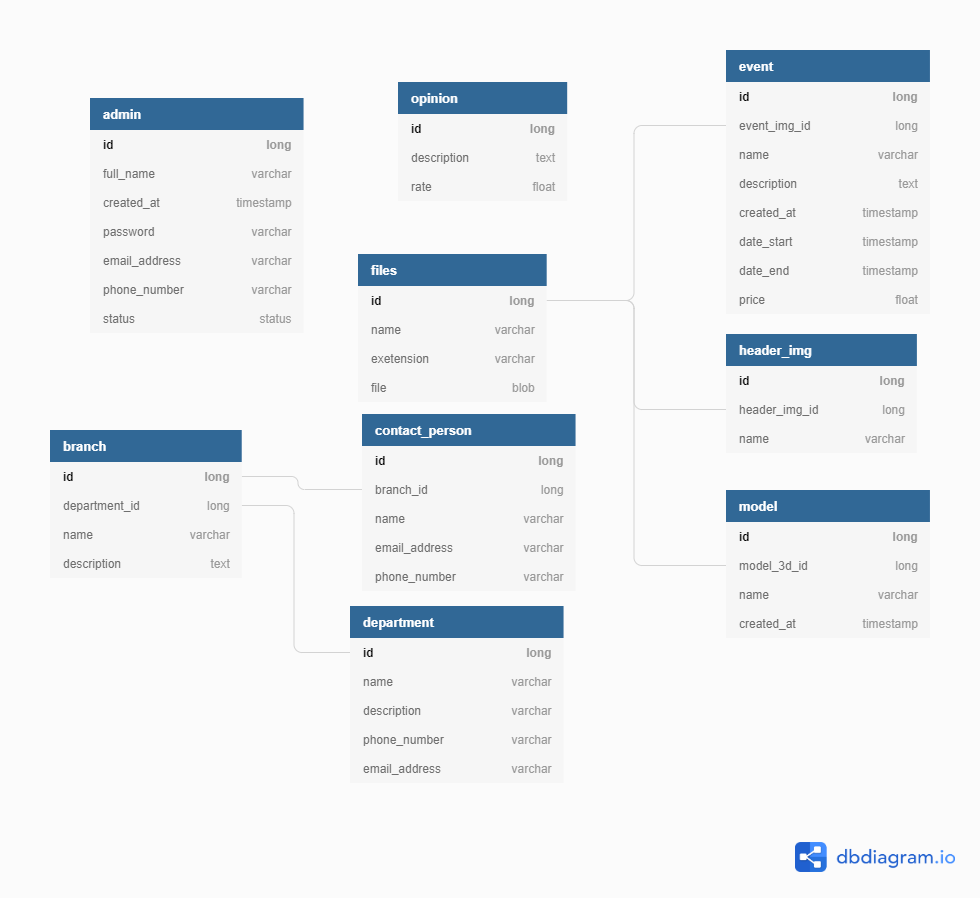
\includegraphics[width=0.5\linewidth]{Sapi3dTour}}
		\caption{Az adatbázis táblák.}
		\label{fig:database}
	\end{figure}

	\paragraph{}
	Az adatbázis megtervezés után, neki fogtam a backend részt elkezdeni. Ehhez Spring Bootot használtam ami megkönnyíti az adatbázis létrehozásának folyamatát. A kódot Java-ban kell írni és minden tábla egy osztálynak felel meg. A Spring Boot tanulmányozása során jöttem rá, hogy mennyire oda kell figyelni a különböző annotációkra. Kis idő elteltével elsajátítottam a Spring Boot struktúráját és ezt használva felépítettem a backend rész első fázisát. Az adatbázis egyelőr PostgreSQL-ben van létrehozva viszont a Spring segítségével gyorsan bármely adatbázissal lehet kapcsolatot teremteni.
	\paragraph{}
	Mindeközben fejlesztettem a frontend részt is. Eljött az a pillanat hogy kapcsolatot kellett teremtenem a frontend és a backend rész között, amelyet hamar sikerült elvégeznem. Így már tudott kommunikálni a frontend a backenddel vagyis a frontendre az adatbázisban szereplő adatok eljutottak és jelentek meg a weboldalon. 
	\paragraph{}
	A következő részben látható lesz képek formájában a forntend rész haladata. Az első részben bemutatnám, hogy a nem általános felhasználók mit látnak. Első sorban a menürendszerrel kezdeném. Ha már be van jelentkezve egy felhasználó akkor a \ref{fig:drawbar} ábrán látható menü rendszerrel fog találkozni. Megfigyelhető, hogy megjelennek a felhasználó adatai és egy gomb amely segítségével tudja módosítani az adatait.Erről képet láthatunk a \ref{fig:changedata} ábrán . Ezek után jönnek a lehetőségek amelyekre rákattintva különböző oldalak jelennek meg.
	\begin{figure}
		\centering
		\frame{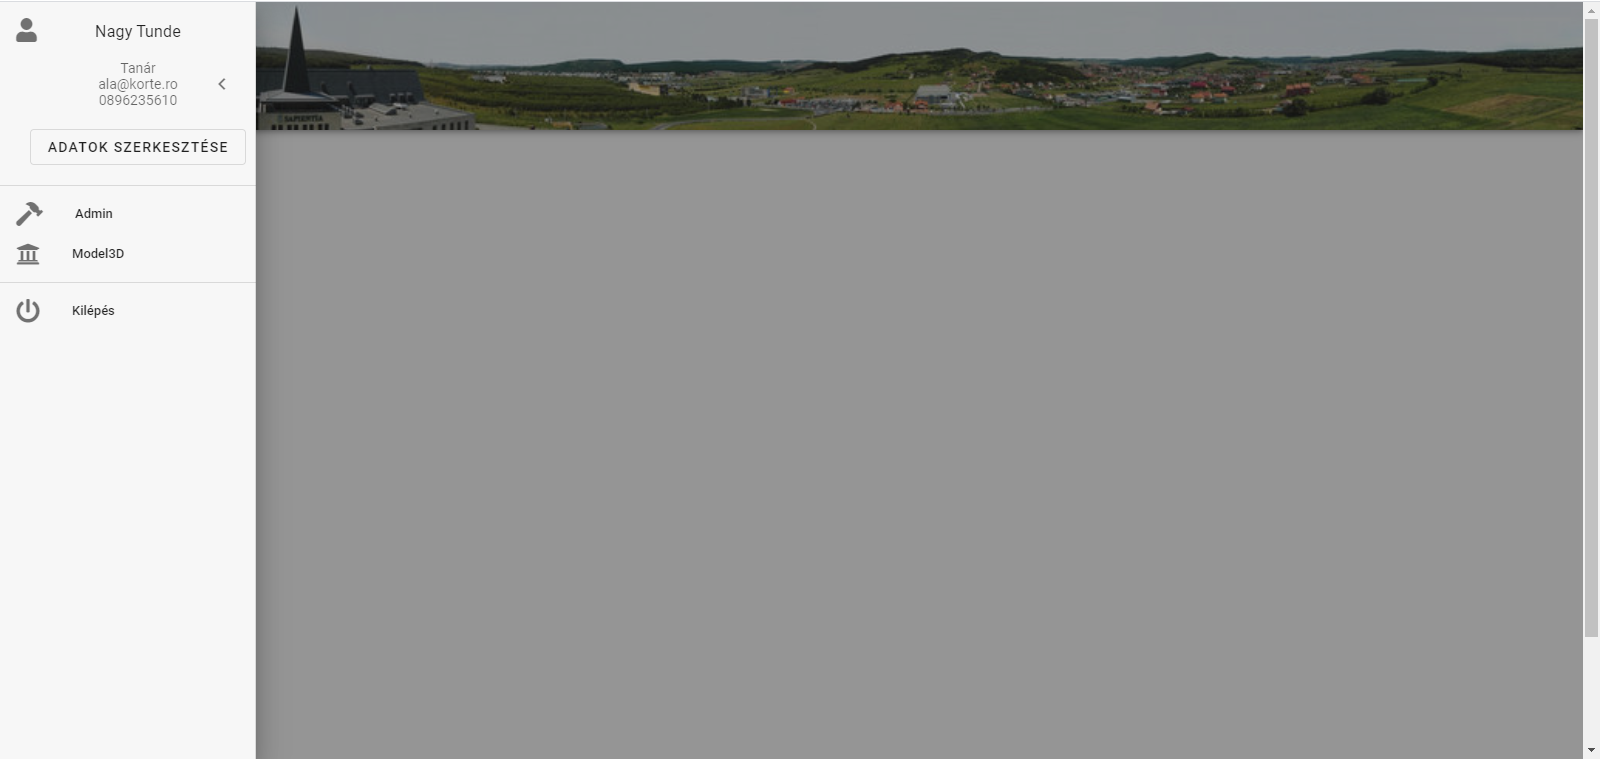
\includegraphics[width=0.8\linewidth]{drawbar}}
		\caption{A nem általános felhasználók menü rendszere}
		\label{fig:drawbar}
	\end{figure}
	\begin{figure}
		\centering
		\frame{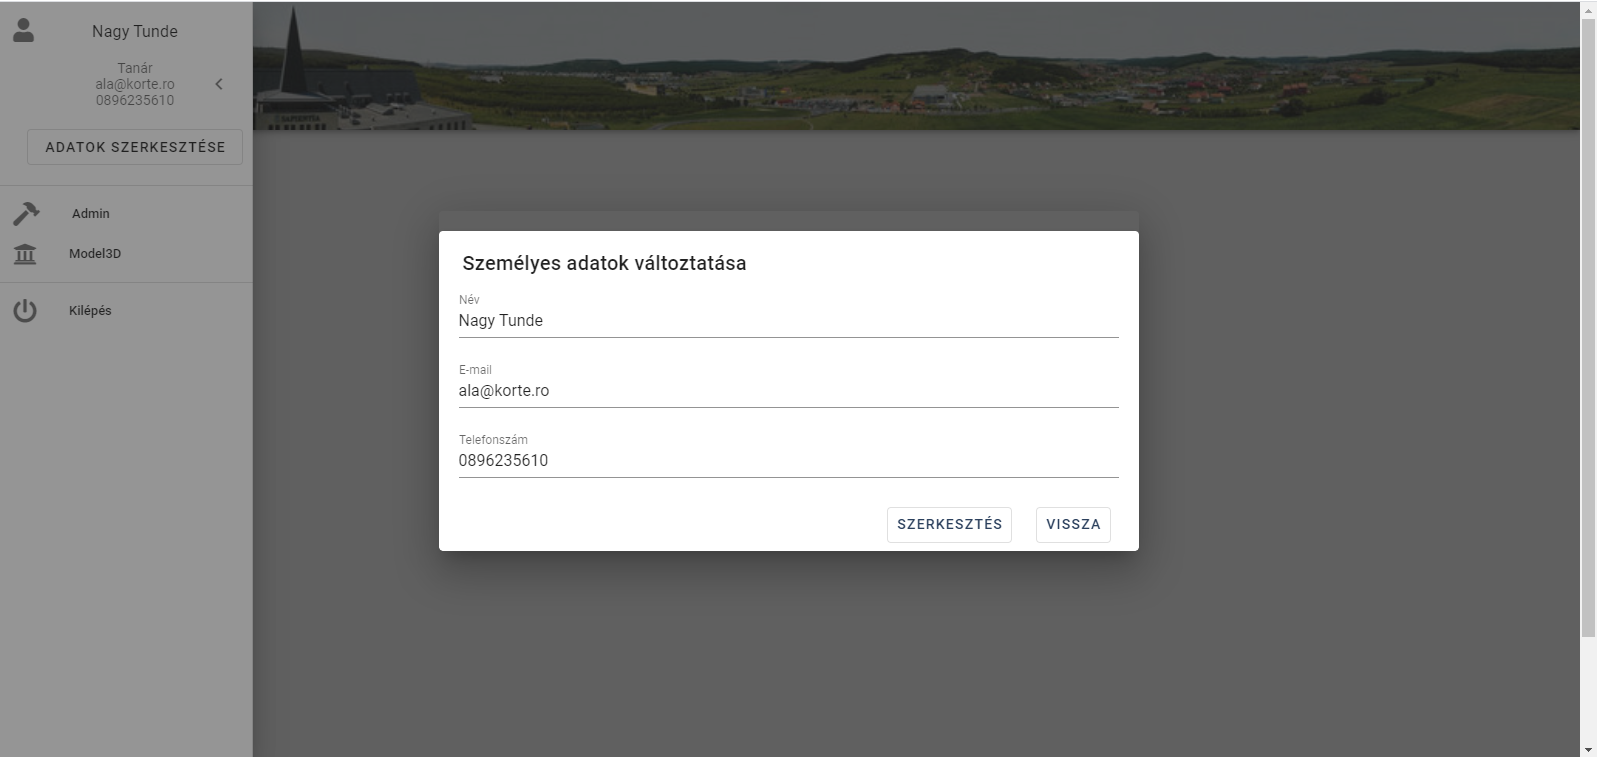
\includegraphics[width=0.8\linewidth]{changedata}}
		\caption{A nem általános felhasználók adatainak módosítása}
		\label{fig:changedata}
	\end{figure}
	
	\paragraph{}
	A menürendszer első opcióját választva vagyis az Admin opciót akkor előjönnek azok a funkcionalitások, amelyeket eltud végezni a felhasználó annak függvényében hogy milyen joggal rendelkezik. Egyelőre csak az új felhasználók hozzáadása működik, amelyhez csak annyit kell tennünk, hogy beírjuk az adatokat és ráklikkelünk a HOZZÁADÁS gombra. Ez által bekerül az új felhasználó az adatbázisba. Erről az oldalról a \ref{fig:admin} ábrán láthatunk egy képet. Az utolsó menü pont a kijelentkezés gomba amely segítségével a felhasználó ki  tud jelentkezni és vissza kerül arra az oldalra amelyet már minden felhasználó képes látni.
	\begin{figure}
		\centering
		\frame{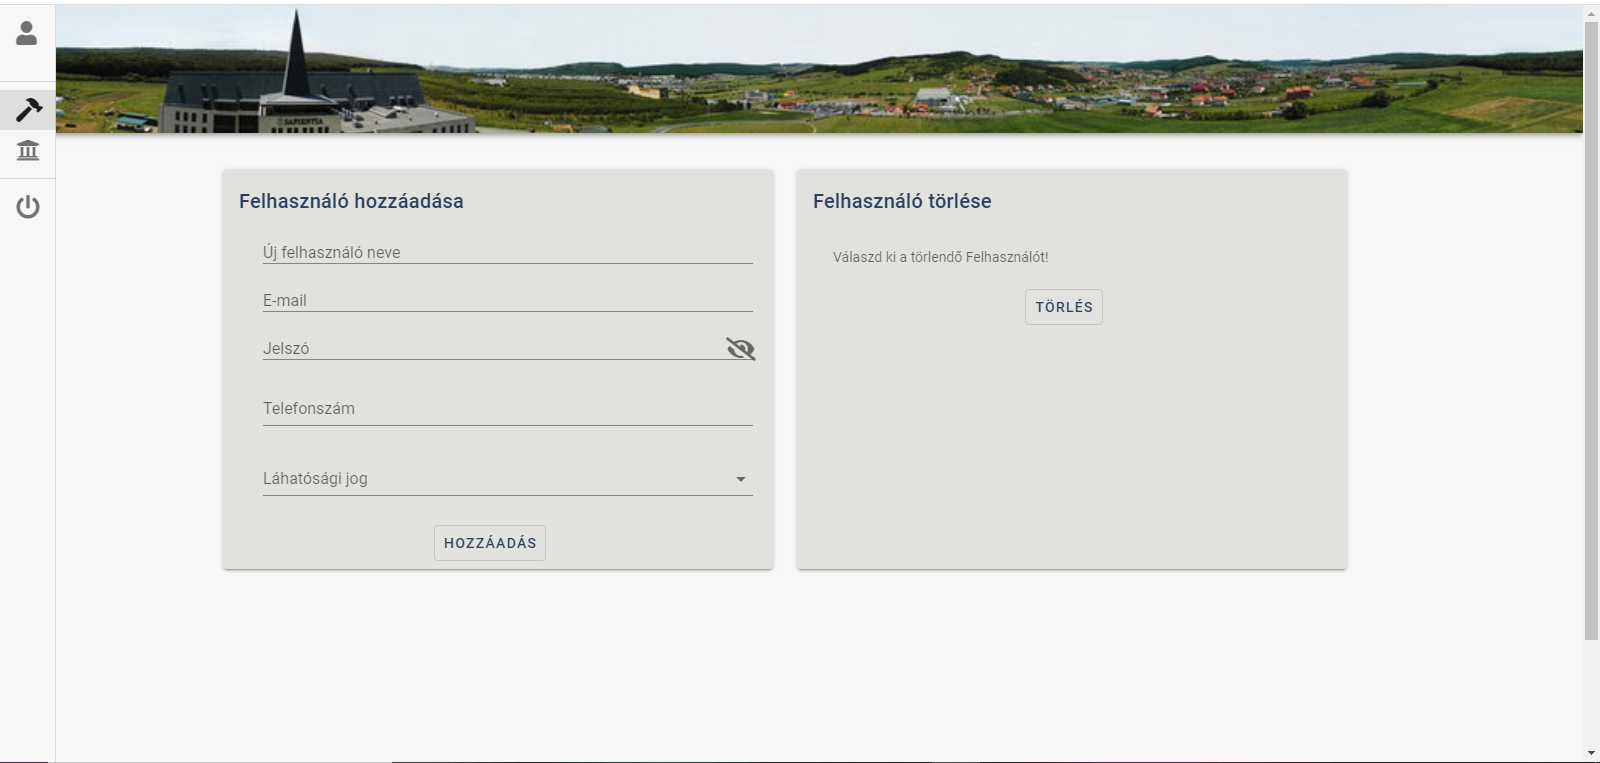
\includegraphics[width=0.8\linewidth]{admin}}
		\caption{A nem általános felhasználók által használt különleges funkciók}
		\label{fig:admin}
	\end{figure}
	
	\paragraph{}
	A következőkben azokat az elemeket mutatnám meg amelyeket minden felhasználó képes látni. Egyelőre csak egy ilyen oldal készült el és ez sem végeleges. Ezen az oldalon látható egy 3D modell amelyet a társam készített el. Megtekinthető a \ref{fig:modell} ábrán. Ezen kívül észrevehető, hogy ha nem vagyunk bejelentkezve akkor egy kicsivel másabb menürendszer jelenik meg. Ezt megtudjuk nézni a \ref{fig:drawbarevery} ábrán. A struktúra hasonló viszont itt nem jelennek meg a felhasználók adatai ámbár megjelenik a Bejelentkezés menüpont ahol be tudnak jelentkezni a felhasználók. Ez tulajdonképpen az útválasztás(rout) folyamaton belül oldódott meg. Egy útválasztás van és azon belül két nagyobb csoportra lett felosztva, hogy ki melyik oldalt láthatja. 
	
	\begin{figure}
		\centering
		\frame{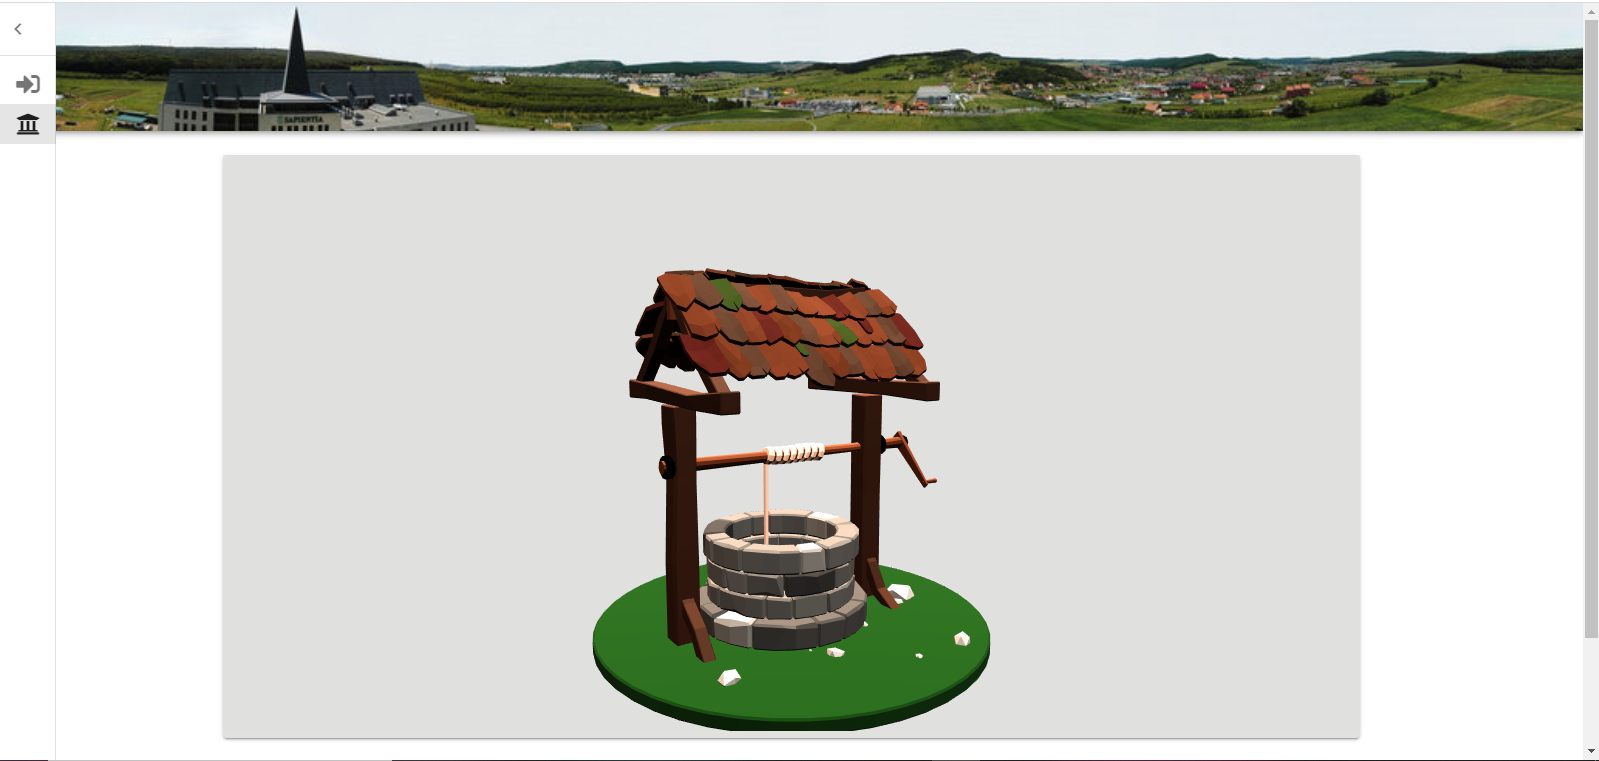
\includegraphics[width=0.8\linewidth]{modell}}
		\caption{A 3D modell kép minden felhasználó számára}
		\label{fig:modell}
	\end{figure}

	\begin{figure}
		\centering
		\frame{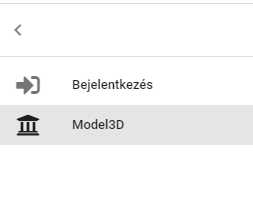
\includegraphics[width=0.8\linewidth]{drawbarevery}}
		\caption{Minden felhasználó által látható menürendszer}
		\label{fig:drawbarevery}
	\end{figure}
	
	\paragraph{}
	Az alkalmazást egyelőre web felületen készítem el, mivel így a különböző eszközökön nem kell különbséget tenni. Nem kell megírni külön Android vagy IOS rendszerrel rendelkező mobiltelefonok nyelvére. A web felületre írt oldalakat megtudja nyitni az Androiddal és IOS rendszerre rendelkező ember is mivel nem kell külön alkalmazást letölteni. Ezen kívül egy weboldal elérhető számítógépeken is. Fejlesztési lehetőségnek persze ott tartom azt is, hogy majd ne csak web applikáció legyen hanem Android meg IOS is. Mindkettőt hasznosnak tartom mivel világunkban a telefonok használata nagyon népszerű. 
	
	\newpage
	
	\section{Összefoglaló}
	\paragraph{}
	Az elmúlt nyár alatt ennyire sikerült az államvizsga projektemet fejlesztenem. Továbbra is törekszem, hogy minél jobban gyorsabban megoldjam a felmerülő problémákat. Folyamatosan próbálok ötletelni minél jobb és kreatívabb megoldásokról annak érdekében, hogy az alkalmazás hasznos legyen mint az egyetem és a diákok részére is. Úgy gondolom a nyár alatt elég sok mindent megtanultam, tapasztaltam a különböző rendszerekkel, technológiákkal kapcsolatban. Ezen tapasztalataimat nagy örömmel fogadtam és tudom, hogy majd a jövőbeni életemben is feltudom használni őket.
	
	\newpage
	
	\bibliographystyle{plainnat}
	\bibliography{nyarigyakbeszallamdol}	 
	
\end{document}